\providecommand{\home}{../../../..}
\documentclass[\home/main.tex]{subfiles}
\usetikzlibrary[arrows,snakes,backgrounds]
\usetikzlibrary{calc,positioning}

\begin{document}

% ===================
%     PID BOX
% ===================

\newsavebox{\PIDBox}

\newcommand{\scaledPID}[2]{\resizebox{#1}{#2}{\usebox{\PIDBox}}}
\newcommand{\scaledPIDWidth}[1]{\resizebox{#1}{!}{\usebox{\PIDBox}}}
\newcommand{\scaledPIDHeight}[1]{\resizebox{!}{#1}{\usebox{\PIDBox}}}

\sbox{\PIDBox}{%
\begin{tikzpicture}[>=latex',every node/.append style=
    {font=\scriptsize},node distance=5mm]

    \tikzset{
        %   pinstyle/.style={pin edge={to-,thin,black}}, % you have another one below
           block/.style = {draw, rectangle,
               minimum height=1cm,
               align = center
            %   minimum width=2cm
           },
           input/.style = {coordinate,node distance=1cm},
           output/.style = {coordinate,node distance=1cm},
           arrow/.style={draw, -latex,node distance=2cm},
           pinstyle/.style = {pin edge={latex-, black,node distance=2cm}},
           sum/.style = {draw, circle, node distance=1cm},
           gain/.style = {
             regular polygon, regular polygon sides=3,
             draw, fill=white, text width=1em,
             inner sep=0mm, outer sep=0mm,
             shape border rotate=-90
           },
           dot/.style={circle,fill,draw,inner sep=0pt,minimum size=3pt}
         }

    %DEFINIZIONE BLOCCHI
    \node [input, name=input] {};
    \node [sum, right=of input] (speed_sum) {};
    \node [dot, right=8mm of speed_sum] (snodo1) {};
    \node [gain, above right=7mm and 5mm of snodo1] (Kp) {$K_{p}$};
    \node [gain, below right=7mm and 5mm of snodo1] (Ki) {$K_{i}$};

    \node [block,right=of Ki] (integrator) {$\frac{1}{s}$};
    \node [sum, xshift=7mm] at (snodo1-|integrator) (control_sum) {};
    \node [gain, right=1cm of control_sum] (Kc) {$K_{c}$};
    \node [block, right=8mm of Kc] (system) {$L(s)$};
    \node [output, right=of system] (output) {};


        %DEFINIZIONE COLLEGAMENTI IN CATENA DIRETTA
    \begin{scope}[auto]
    \draw [->] (input) -- node {$\omega_{M}^{\mathrm{dir}}(s)$} (speed_sum);
    \draw [->] (speed_sum) -- node {$E_{v}(s)$}(snodo1);
    \draw [->] (snodo1) |- (Kp);
    \draw [->] (snodo1) |- (Ki);
    \draw [->] (Ki) -- (integrator);
    \draw [->] (Kp) -| (control_sum) node[very near end,swap] {$-$};
    \draw [->] (integrator) -| (control_sum) node[very near end] {$-$};
    \draw [->] (control_sum) -- (Kc);
    \draw [->] (Kc) -- node [align=center] {$I(s)$}(system);
    \draw [->] (system) -- node [name=motor_speed] {$s\theta_{M}(s)$}
        (output);
    \end{scope}

        %DEFINIZIONE COLLEGAMENTI FEEDBACK
    \draw [->] (motor_speed) -- ++ (0,-2.5) -| node [pos=0.99,right] {$-$} node[dot,pos=0.22] (snodo2) {}
    (speed_sum);
    \node [dot] at (motor_speed.south) {};

    \draw [->] (snodo2) -- ++(0,0.5) node[above,draw] (KiKd) {$K_i.K_d$};
    \draw [->] (KiKd) -- ++(0,1) -- node[above,pos=0.5] {$-$}(control_sum);

\end{tikzpicture}
}

% ===================
%     COMPLETE FIG
% ===================

\begin{tikzpicture}
    \def\picMinWidth{5cm}
    \def\picMinHeight{4.0cm}

    \tikzset{
        block/.append style={node distance=35mm,minimum width=3.5cm},
        picture/.style={block, node distance=6cm, fill=white, draw=white,minimum width=\picMinWidth, minimum height=\picMinHeight, text width=\picMinWidth,},
        preSpacedDash/.style={preSpaced, dashed,draw=black!50, thin},
        annot/.style={text width=4em, text centered},
    }

% pictures: see https://rail.eecs.berkeley.edu/deeprlcourse/static/slides/lec-1.pdf slide 23

    \node[block] (obs) {Observation};
    % This has to be a picture that shows the cameras on Douglas while baxter is in scene with the clothing setup.
    %  Clothing setup is the standard folding setup we envision: some unfolded cltohing in the basket, folded cloths on the right and a crumbled cloth in front of baxter. 
    % The keyword here is observation so we want the camera to be the main focus, so I guess a topdown view or at least a "high, elevated" view would be best. 
    \node[picture] (obs_pic) [right of=obs] {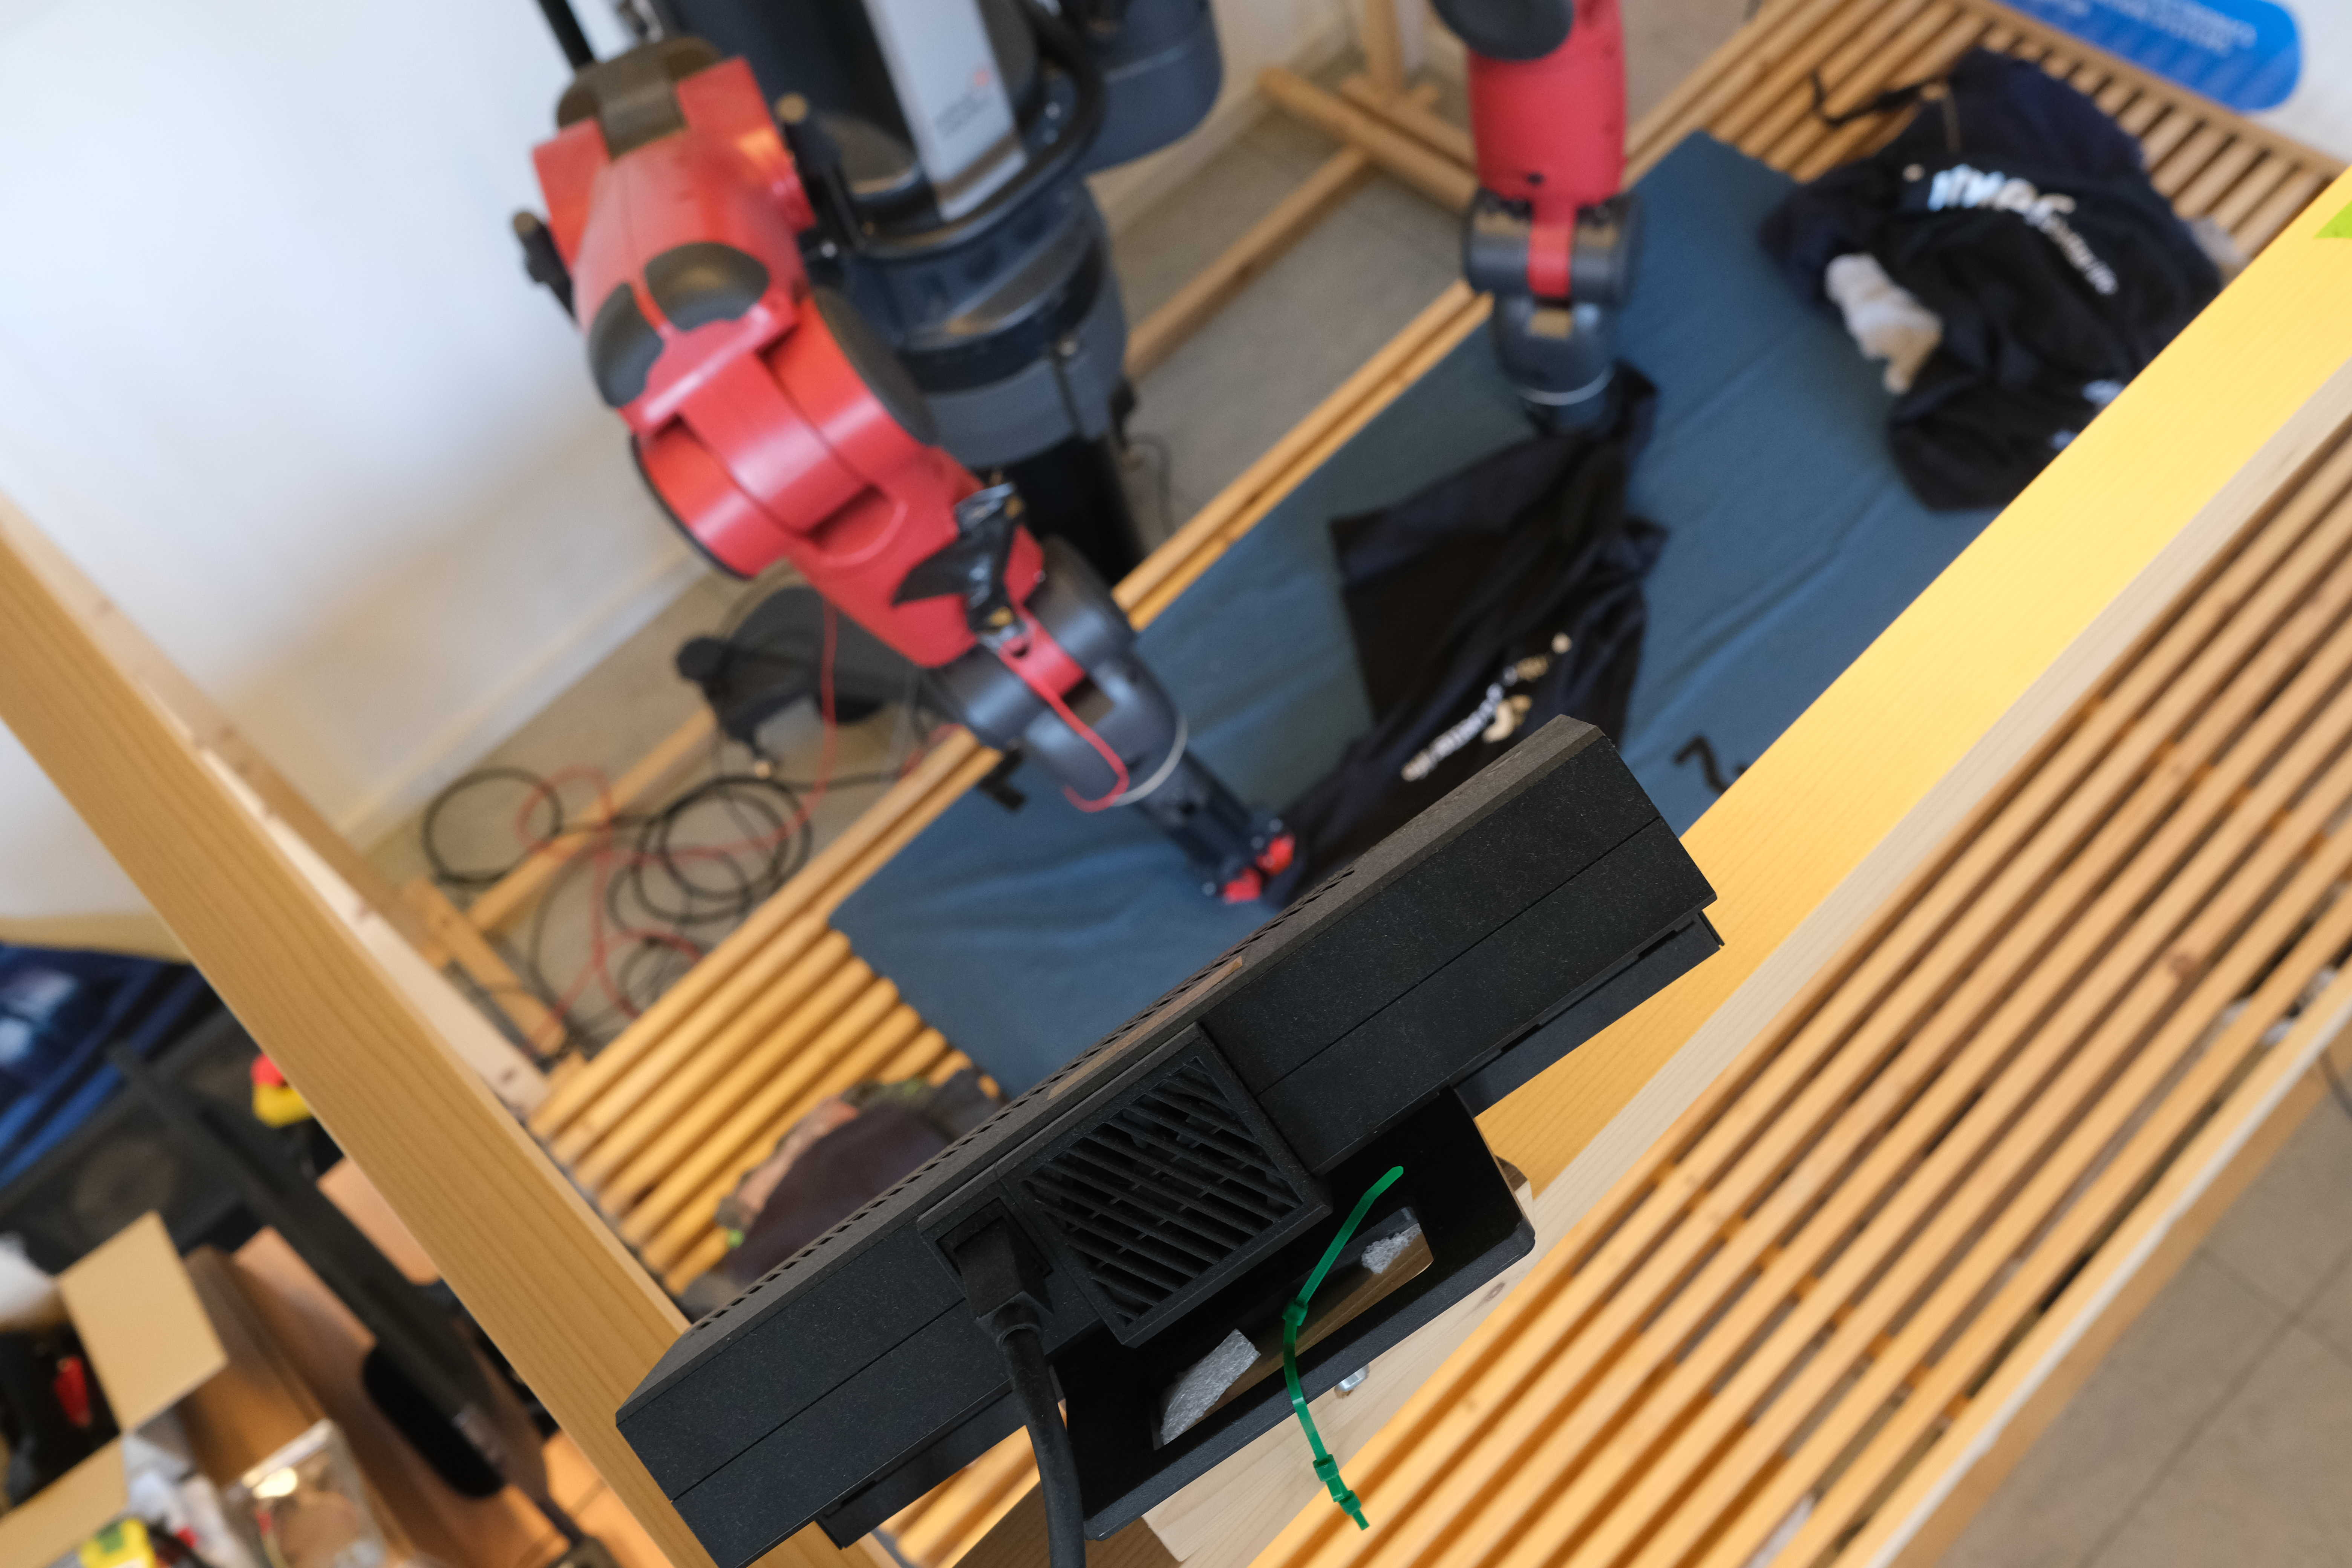
\includegraphics[width=\picMinWidth, height=\picMinHeight]{\home/chapters/02-sota/figures/baxter_camera_obs_50p.jpg}}
        edge[preSpacedDash] node[midway,above=0.5pt,]{\tiny{\textcolor{black!50}{example}}} (obs);

    \node[block] (state) [below of=obs] {State estimation}
        edge[preSpacedArrow] (obs);
    % This picture has to be a zoom in from the point of view of one the Douglas cameras and annotate the baxter end-effector his hand wrench and the keypoitn detection of the cloth
    \node[picture] (state_pic) [right of=state] {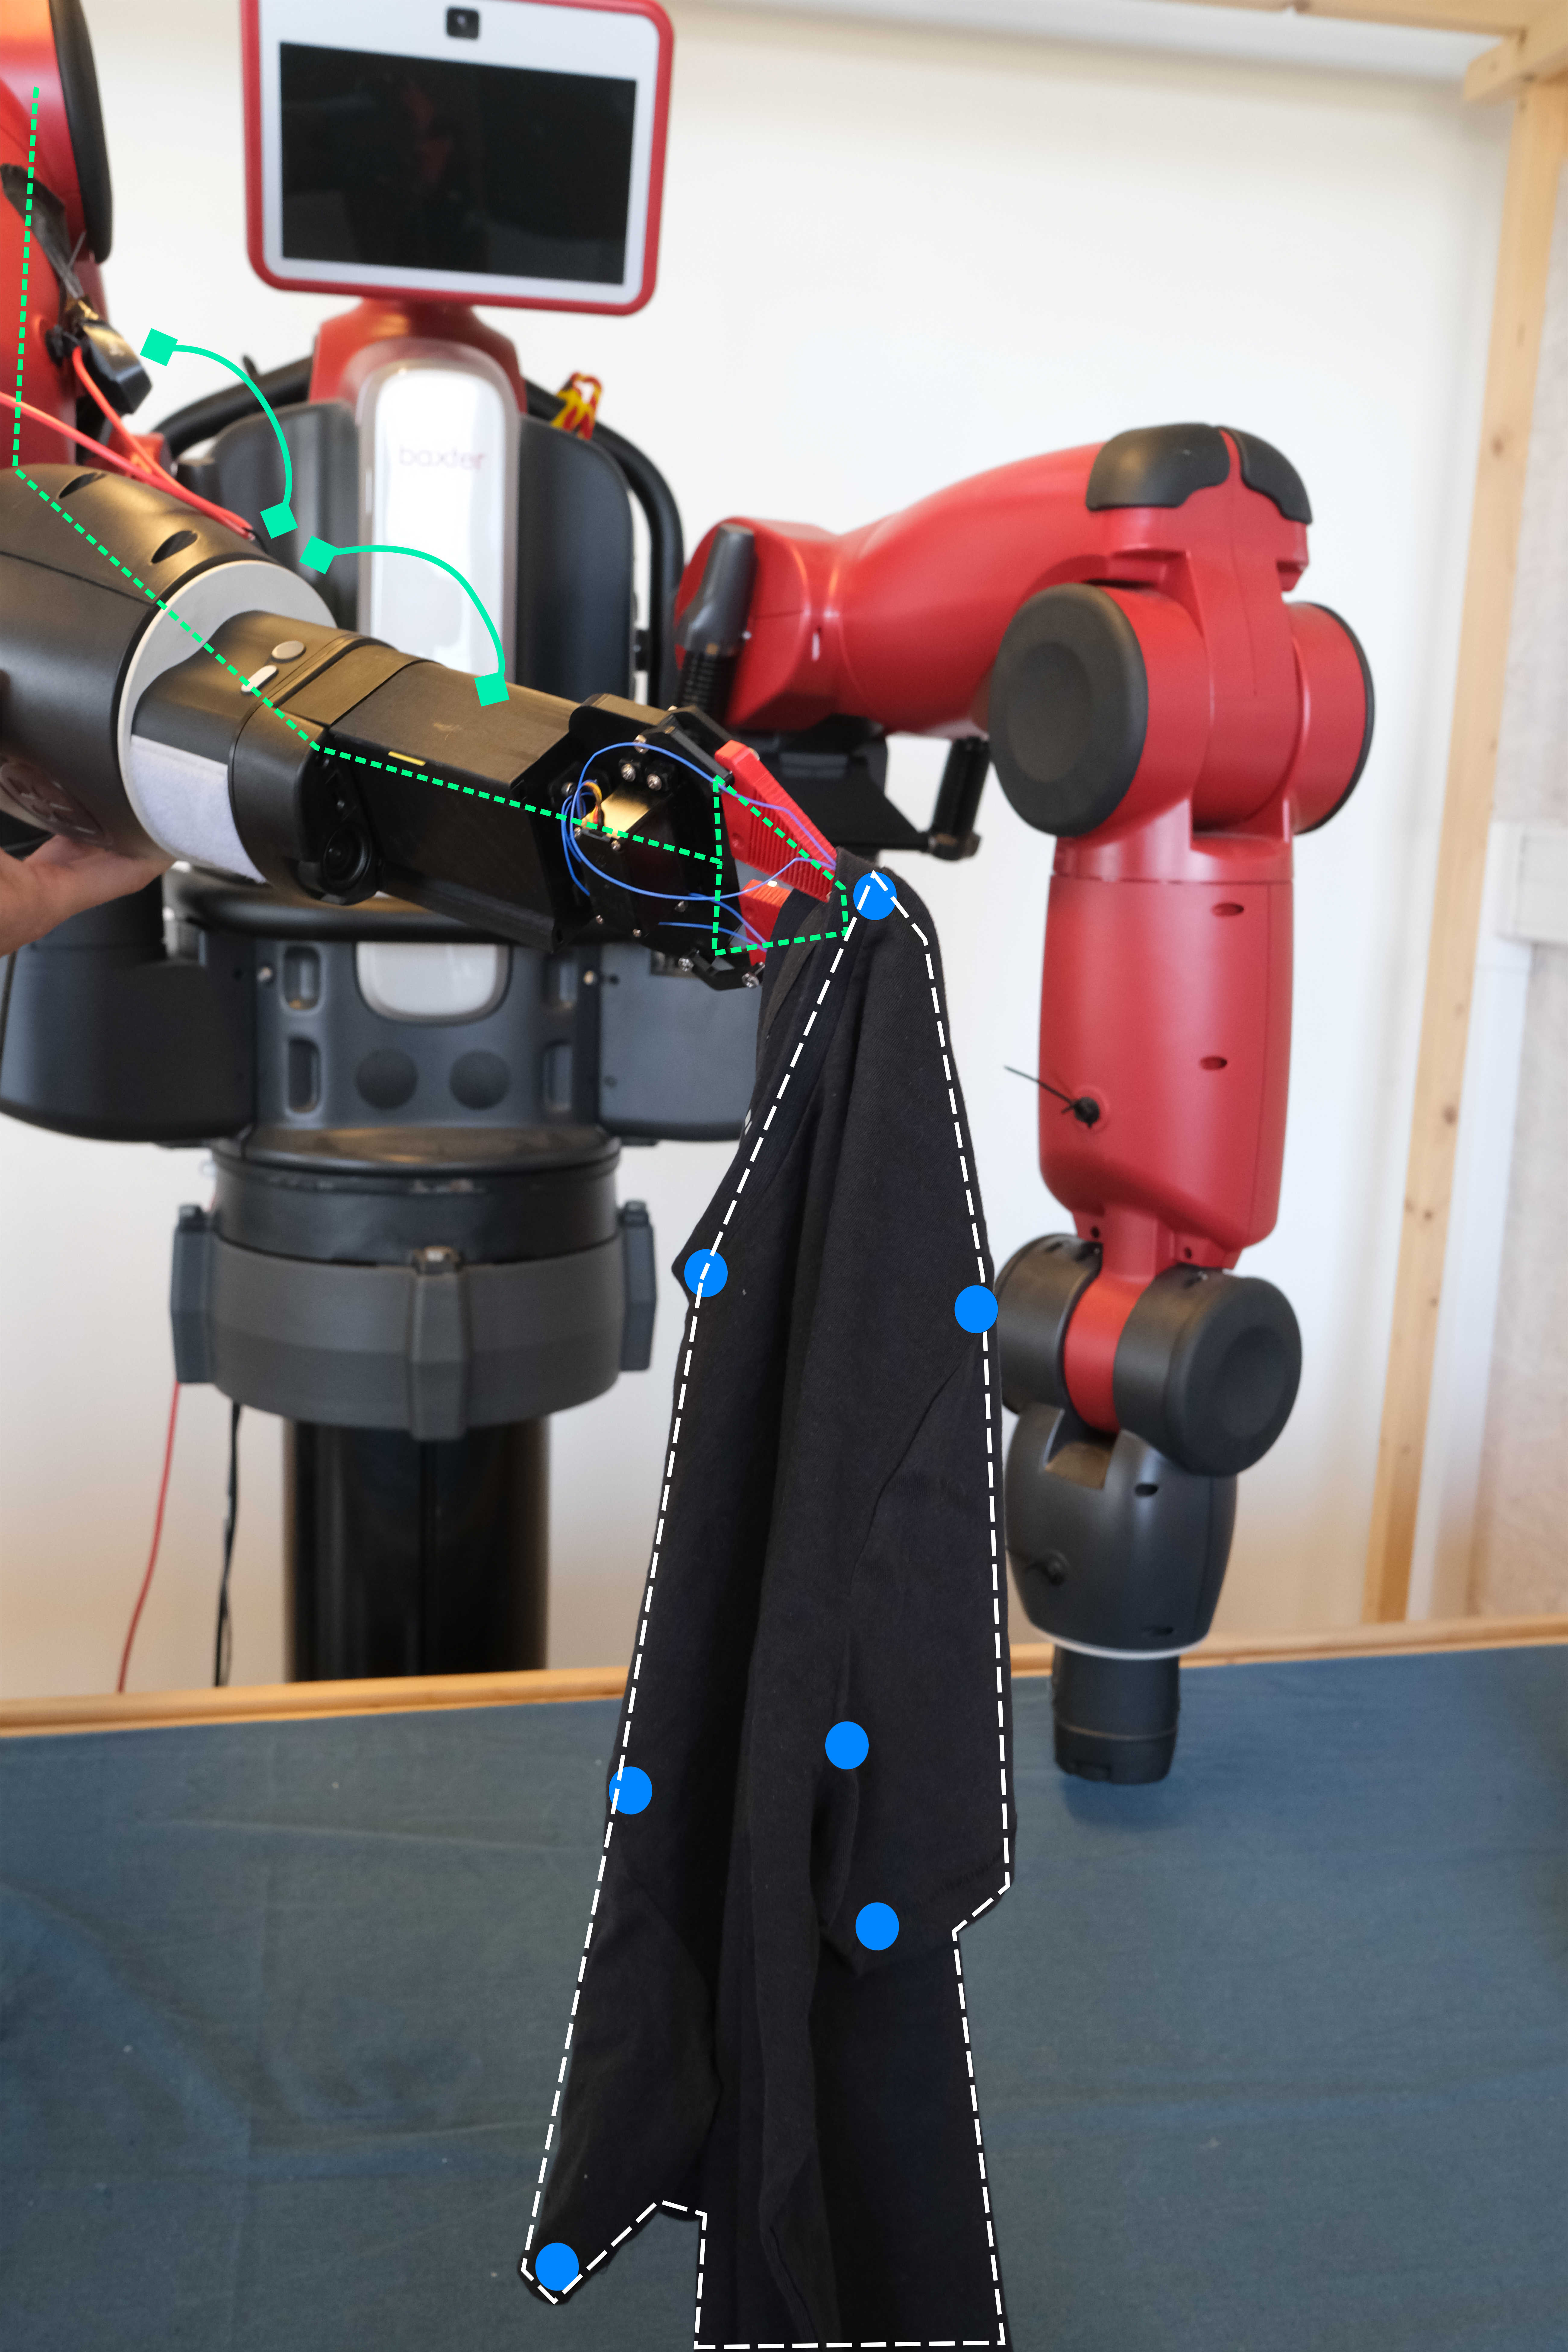
\includegraphics[width=\picMinWidth, height=\picMinHeight]{\home/chapters/02-sota/figures/baxter_state_example_annotated.jpg}}
        edge[preSpacedDash] node[midway,above=0.5pt,]{\tiny{\textcolor{black!50}{example}}} (state);

    \node[block] (modeling) [below of=state,align=center] {Modeling and\\prediction}
        edge[preSpacedArrow] (state);
    %  This picture has to be from a cloth simulator that is folding midway 
    \node[picture] (modeling_pic) [right of=modeling] {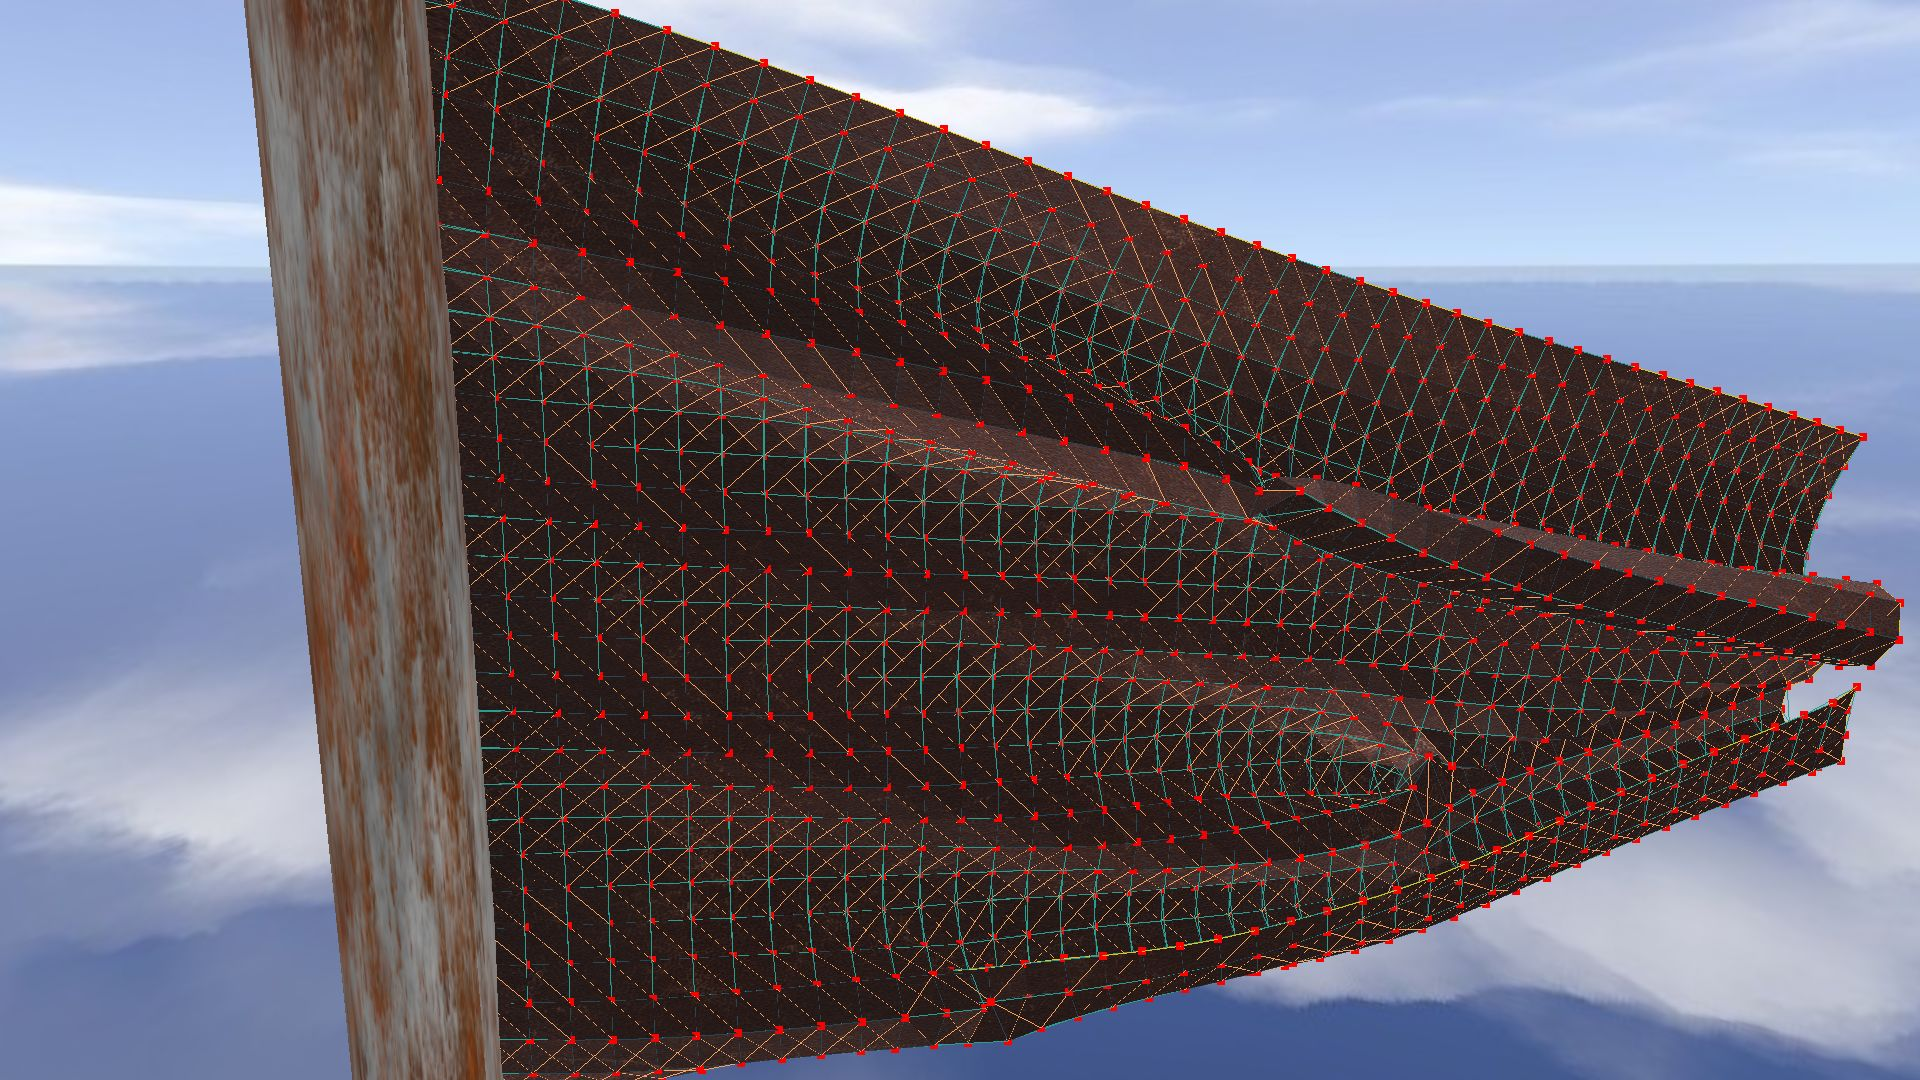
\includegraphics[width=\picMinWidth, height=\picMinHeight]{cloth_state_80p.jpg}}
        edge[preSpacedDash] node[midway,above=0.5pt,]{\tiny{\textcolor{black!50}{example}}} (modeling);

    \node[block] (planning) [below of=modeling] {Planning}
        edge[preSpacedArrow] (modeling);
    % This picture has to be Baxter in moveit environment, put his arms somewhere and draw lines of the trajectory where they came from
    \node[picture] (planning_pic) [right of=planning] {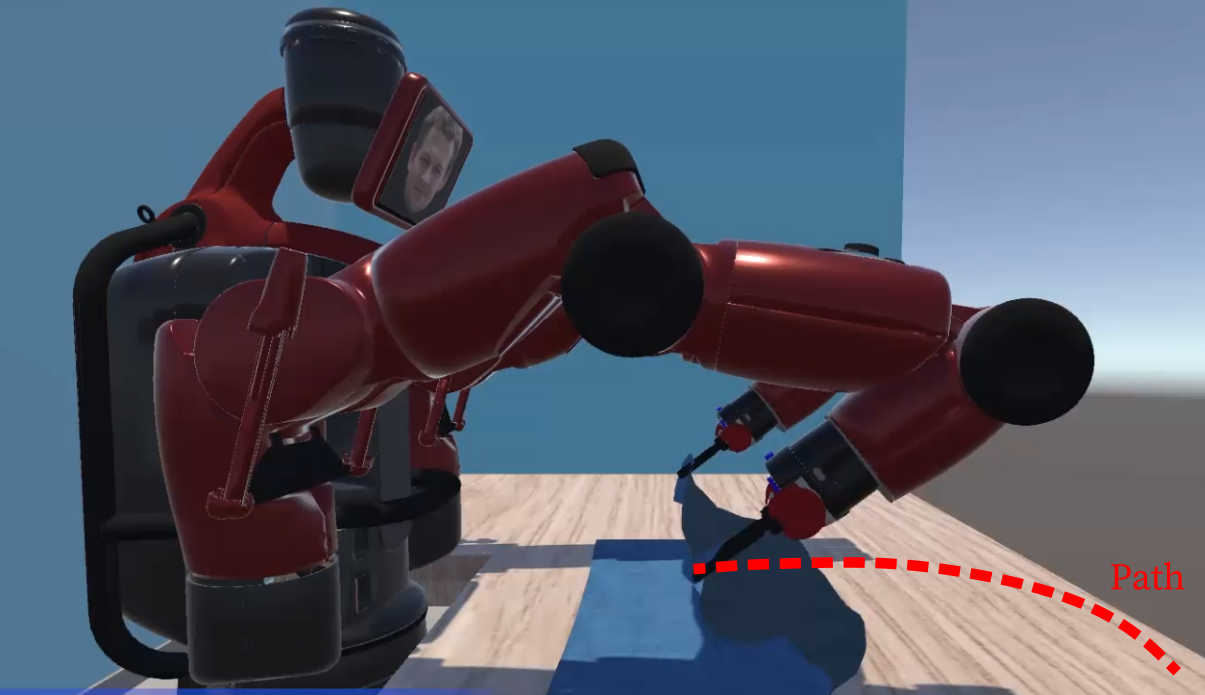
\includegraphics[width=\picMinWidth, height=\picMinHeight]{baxter_path_planning.jpg}}
        edge[preSpacedDash]  node[midway,above=0.5pt,]{\tiny{\textcolor{black!50}{example}}} (planning);
    
    \node[block] (control) [below of=planning] {Control}
        edge[preSpacedArrow] (planning);
    \node[picture] (control_pic) [right of=control] {\scaledPIDWidth{\picMinWidth}}
        edge[preSpacedDash] node[midway,above=0.5pt,]{\tiny{\textcolor{black!50}{example}}} (control);

\end{tikzpicture}

\end{document}
